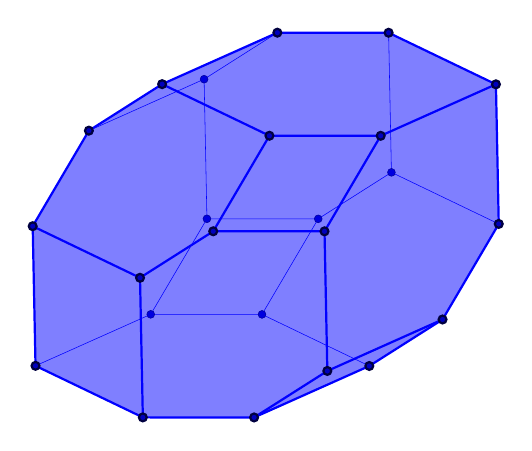
\begin{tikzpicture}%
	[x={(0.681462cm, -0.327528cm)},
	y={(0.731633cm, 0.326817cm)},
	z={(-0.017949cm, 0.886519cm)},
	scale=1.000000,
	back/.style={very thin},
	edge/.style={color=blue, thick},
	facet/.style={fill=blue,fill opacity=0.500000},
	vertex/.style={inner sep=1pt,circle,draw=blue!25!black,fill=blue!75!black,thick,anchor=base}]
%
%
%% Coordinate of the vertices:
%%
\coordinate (-0.16667, 2.33333, -0.16667) at (-0.16667, 2.33333, -0.16667);
\coordinate (1.16667, 0.66667, -1.83333) at (1.16667, 0.66667, -1.83333);
\coordinate (1.83333, -0.66667, 0.83333) at (1.83333, -0.66667, 0.83333);
\coordinate (1.83333, 2.33333, -0.16667) at (1.83333, 2.33333, -0.16667);
\coordinate (1.83333, 1.33333, -1.16667) at (1.83333, 1.33333, -1.16667);
\coordinate (1.83333, 2.33333, 1.83333) at (1.83333, 2.33333, 1.83333);
\coordinate (1.83333, -0.66667, -1.16667) at (1.83333, -0.66667, -1.16667);
\coordinate (1.83333, 0.33333, 1.83333) at (1.83333, 0.33333, 1.83333);
\coordinate (1.16667, -1.33333, -1.83333) at (1.16667, -1.33333, -1.83333);
\coordinate (0.83333, -0.66667, 1.83333) at (0.83333, -0.66667, 1.83333);
\coordinate (0.83333, -1.66667, 0.83333) at (0.83333, -1.66667, 0.83333);
\coordinate (0.16667, -2.33333, 0.16667) at (0.16667, -2.33333, 0.16667);
\coordinate (-0.83333, 0.66667, -1.83333) at (-0.83333, 0.66667, -1.83333);
\coordinate (0.16667, -2.33333, -1.83333) at (0.16667, -2.33333, -1.83333);
\coordinate (-1.16667, -0.66667, 1.83333) at (-1.16667, -0.66667, 1.83333);
\coordinate (-1.16667, 1.33333, 1.83333) at (-1.16667, 1.33333, 1.83333);
\coordinate (-0.16667, 2.33333, 1.83333) at (-0.16667, 2.33333, 1.83333);
\coordinate (-0.83333, 1.66667, -0.83333) at (-0.83333, 1.66667, -0.83333);
\coordinate (-1.83333, 0.66667, -0.83333) at (-1.83333, 0.66667, -0.83333);
\coordinate (-1.83333, 0.66667, 1.16667) at (-1.83333, 0.66667, 1.16667);
\coordinate (-1.83333, -1.33333, 1.16667) at (-1.83333, -1.33333, 1.16667);
\coordinate (-1.83333, -2.33333, -1.83333) at (-1.83333, -2.33333, -1.83333);
\coordinate (-1.83333, -2.33333, 0.16667) at (-1.83333, -2.33333, 0.16667);
\coordinate (-1.83333, -0.33333, -1.83333) at (-1.83333, -0.33333, -1.83333);
%%
%%
%% Drawing edges in the back
%%
\draw[edge,back] (-0.16667, 2.33333, -0.16667) -- (1.83333, 2.33333, -0.16667);
\draw[edge,back] (-0.16667, 2.33333, -0.16667) -- (-0.16667, 2.33333, 1.83333);
\draw[edge,back] (-0.16667, 2.33333, -0.16667) -- (-0.83333, 1.66667, -0.83333);
\draw[edge,back] (1.16667, 0.66667, -1.83333) -- (-0.83333, 0.66667, -1.83333);
\draw[edge,back] (-0.83333, 0.66667, -1.83333) -- (-0.83333, 1.66667, -0.83333);
\draw[edge,back] (-0.83333, 0.66667, -1.83333) -- (-1.83333, -0.33333, -1.83333);
\draw[edge,back] (-1.16667, 1.33333, 1.83333) -- (-1.83333, 0.66667, 1.16667);
\draw[edge,back] (-0.83333, 1.66667, -0.83333) -- (-1.83333, 0.66667, -0.83333);
\draw[edge,back] (-1.83333, 0.66667, -0.83333) -- (-1.83333, 0.66667, 1.16667);
\draw[edge,back] (-1.83333, 0.66667, -0.83333) -- (-1.83333, -0.33333, -1.83333);
\draw[edge,back] (-1.83333, 0.66667, 1.16667) -- (-1.83333, -1.33333, 1.16667);
\draw[edge,back] (-1.83333, -2.33333, -1.83333) -- (-1.83333, -0.33333, -1.83333);
%%
%%
%% Drawing vertices in the back
%%
\node[vertex,back] at (-0.16667, 2.33333, -0.16667)     {};
\node[vertex,back] at (-0.83333, 0.66667, -1.83333)     {};
\node[vertex,back] at (-0.83333, 1.66667, -0.83333)     {};
\node[vertex,back] at (-1.83333, 0.66667, -0.83333)     {};
\node[vertex,back] at (-1.83333, 0.66667, 1.16667)     {};
\node[vertex,back] at (-1.83333, -0.33333, -1.83333)     {};
%%
%%
%% Drawing the facets
%%
\fill[facet] (1.83333, 1.33333, -1.16667) -- (1.83333, 2.33333, -0.16667) -- (1.83333, 2.33333, 1.83333) -- (1.83333, 0.33333, 1.83333) -- (1.83333, -0.66667, 0.83333) -- (1.83333, -0.66667, -1.16667) -- cycle {};
\fill[facet] (0.83333, -1.66667, 0.83333) -- (1.83333, -0.66667, 0.83333) -- (1.83333, 0.33333, 1.83333) -- (0.83333, -0.66667, 1.83333) -- cycle {};
\fill[facet] (0.16667, -2.33333, -1.83333) -- (1.16667, -1.33333, -1.83333) -- (1.83333, -0.66667, -1.16667) -- (1.83333, -0.66667, 0.83333) -- (0.83333, -1.66667, 0.83333) -- (0.16667, -2.33333, 0.16667) -- cycle {};
\fill[facet] (1.16667, -1.33333, -1.83333) -- (1.16667, 0.66667, -1.83333) -- (1.83333, 1.33333, -1.16667) -- (1.83333, -0.66667, -1.16667) -- cycle {};
\fill[facet] (-0.16667, 2.33333, 1.83333) -- (1.83333, 2.33333, 1.83333) -- (1.83333, 0.33333, 1.83333) -- (0.83333, -0.66667, 1.83333) -- (-1.16667, -0.66667, 1.83333) -- (-1.16667, 1.33333, 1.83333) -- cycle {};
\fill[facet] (-1.83333, -2.33333, 0.16667) -- (0.16667, -2.33333, 0.16667) -- (0.83333, -1.66667, 0.83333) -- (0.83333, -0.66667, 1.83333) -- (-1.16667, -0.66667, 1.83333) -- (-1.83333, -1.33333, 1.16667) -- cycle {};
\fill[facet] (-1.83333, -2.33333, 0.16667) -- (0.16667, -2.33333, 0.16667) -- (0.16667, -2.33333, -1.83333) -- (-1.83333, -2.33333, -1.83333) -- cycle {};
%%
%%
%% Drawing edges in the front
%%
\draw[edge] (1.16667, 0.66667, -1.83333) -- (1.83333, 1.33333, -1.16667);
\draw[edge] (1.16667, 0.66667, -1.83333) -- (1.16667, -1.33333, -1.83333);
\draw[edge] (1.83333, -0.66667, 0.83333) -- (1.83333, -0.66667, -1.16667);
\draw[edge] (1.83333, -0.66667, 0.83333) -- (1.83333, 0.33333, 1.83333);
\draw[edge] (1.83333, -0.66667, 0.83333) -- (0.83333, -1.66667, 0.83333);
\draw[edge] (1.83333, 2.33333, -0.16667) -- (1.83333, 1.33333, -1.16667);
\draw[edge] (1.83333, 2.33333, -0.16667) -- (1.83333, 2.33333, 1.83333);
\draw[edge] (1.83333, 1.33333, -1.16667) -- (1.83333, -0.66667, -1.16667);
\draw[edge] (1.83333, 2.33333, 1.83333) -- (1.83333, 0.33333, 1.83333);
\draw[edge] (1.83333, 2.33333, 1.83333) -- (-0.16667, 2.33333, 1.83333);
\draw[edge] (1.83333, -0.66667, -1.16667) -- (1.16667, -1.33333, -1.83333);
\draw[edge] (1.83333, 0.33333, 1.83333) -- (0.83333, -0.66667, 1.83333);
\draw[edge] (1.16667, -1.33333, -1.83333) -- (0.16667, -2.33333, -1.83333);
\draw[edge] (0.83333, -0.66667, 1.83333) -- (0.83333, -1.66667, 0.83333);
\draw[edge] (0.83333, -0.66667, 1.83333) -- (-1.16667, -0.66667, 1.83333);
\draw[edge] (0.83333, -1.66667, 0.83333) -- (0.16667, -2.33333, 0.16667);
\draw[edge] (0.16667, -2.33333, 0.16667) -- (0.16667, -2.33333, -1.83333);
\draw[edge] (0.16667, -2.33333, 0.16667) -- (-1.83333, -2.33333, 0.16667);
\draw[edge] (0.16667, -2.33333, -1.83333) -- (-1.83333, -2.33333, -1.83333);
\draw[edge] (-1.16667, -0.66667, 1.83333) -- (-1.16667, 1.33333, 1.83333);
\draw[edge] (-1.16667, -0.66667, 1.83333) -- (-1.83333, -1.33333, 1.16667);
\draw[edge] (-1.16667, 1.33333, 1.83333) -- (-0.16667, 2.33333, 1.83333);
\draw[edge] (-1.83333, -1.33333, 1.16667) -- (-1.83333, -2.33333, 0.16667);
\draw[edge] (-1.83333, -2.33333, -1.83333) -- (-1.83333, -2.33333, 0.16667);
%%
%%
%% Drawing the vertices in the front
%%
\node[vertex] at (1.16667, 0.66667, -1.83333)     {};
\node[vertex] at (1.83333, -0.66667, 0.83333)     {};
\node[vertex] at (1.83333, 2.33333, -0.16667)     {};
\node[vertex] at (1.83333, 1.33333, -1.16667)     {};
\node[vertex] at (1.83333, 2.33333, 1.83333)     {};
\node[vertex] at (1.83333, -0.66667, -1.16667)     {};
\node[vertex] at (1.83333, 0.33333, 1.83333)     {};
\node[vertex] at (1.16667, -1.33333, -1.83333)     {};
\node[vertex] at (0.83333, -0.66667, 1.83333)     {};
\node[vertex] at (0.83333, -1.66667, 0.83333)     {};
\node[vertex] at (0.16667, -2.33333, 0.16667)     {};
\node[vertex] at (0.16667, -2.33333, -1.83333)     {};
\node[vertex] at (-1.16667, -0.66667, 1.83333)     {};
\node[vertex] at (-1.16667, 1.33333, 1.83333)     {};
\node[vertex] at (-0.16667, 2.33333, 1.83333)     {};
\node[vertex] at (-1.83333, -1.33333, 1.16667)     {};
\node[vertex] at (-1.83333, -2.33333, -1.83333)     {};
\node[vertex] at (-1.83333, -2.33333, 0.16667)     {};
%%
%%
\end{tikzpicture}